\section{Demonstration}

The CPR demo is provided as a Git repository and associated Docker image that enable the examples to be run on Linux, macOS, and Windows-based systems that have Git, Docker, and GNU Make installed. Each example uses the CPR toolkit to record OS-level provenance information from a run of a different computational workflow, to load a Blazegraph instance with the resulting CPR traces, and to produce a set of reports and visualizations via SPARQL queries.
 
A Makefile in the top directory of the demo repository provides targets for pulling the Docker image from Dockerhub (\commandtext{pull-image}), building the Docker image locally (\commandtext{build-image}), for running the examples (\commandtext{run-examples}), and for deleting all of the reports, visualizations, and other artifacts generated for each example (\commandtext{clean-examples}). Because the expected results are included in the repository, successful reproduction of the example products is demonstrated by issuing the commands \commandtext{make clean-examples} and \commandtext{make run-examples} and confirming that \commandtext{git diff} reports no differences.

Query results and visualizations for each example provide answers to standard questions including:
\begin{enumerate}
\item \emph{What programs and script invocations occur as part of the run?}
\item \emph{What files represent inputs and outputs of the run as a whole?}
\item \emph{What are the input and output data files for each process in the run?}
\item \emph{Which files input to a run are used to produce a particular output file?}
\item \emph{Which run output artifacts are affected by a particular input file?}
\item \emph{What programs contribute to the production of a particular output artifact?}
\end{enumerate}

\begin{figure}[t]
\begin{verbatim}
    #!/bin/bash
    cat inputs/i1.txt inputs/i2.txt > temp/t12.txt
    cat inputs/i1.txt inputs/i2.txt inputs/i3.txt > temp/t123.txt
    cat inputs/i4.txt > temp/t4.txt
    cat temp/t12.txt > outputs/o12.txt
    cat temp/t123.txt temp/t4.txt > outputs/o1234.txt
    cat temp/t4.txt > outputs/o4.txt
\end{verbatim}
\vspace*{-1.5em}  % BL: fine-tune as needed 
        \caption{Workflow script.}
      \end{figure}

The example computations range from trivial and domain-independent, to relatively complex and domain-specific. An example of minimal complexity that still demonstrates key capabilities of CPR is illustrated in Figure \ref{fig:cpr-example}. A simple bash script invokes the \commandtext{cat} command six times on different combinations of three input files to produce three intermediate files and three final output files. The run profile shown allows CPR to identify the data files (and to ignore system files needed to run the script but irrelevant to the questions a verifier typically asks).  The visualizations satisfying queries 2 and 3 are included for a run of this script and depicts the answers as dataflow graphs. We expect the visualization answering query 3 to be the main CPR artifact a verifier will use to compare the record of execution with the description of the computation in a paper. Visualizations answering queries 4 and 5 can be considered to be subgraphs of the visualization for query 3 limited to nodes and edges relevant to a single output or input file. 

\begin{figure}[th]
        \centering
\begin{subfigure}[b]{0.20\linewidth}
\begin{verbatim}
roles:
  os:
    - /etc
    - /lib
    - /usr/lib
  sw:
    - /usr/bin
  in:
    - ./inputs
  out:
    - ./outputs
  tmp:
    - ./temp
\end{verbatim}
            \caption{Run profile.}
        \end{subfigure}
\hfill
        \begin{subfigure}[b]{0.69\linewidth}
            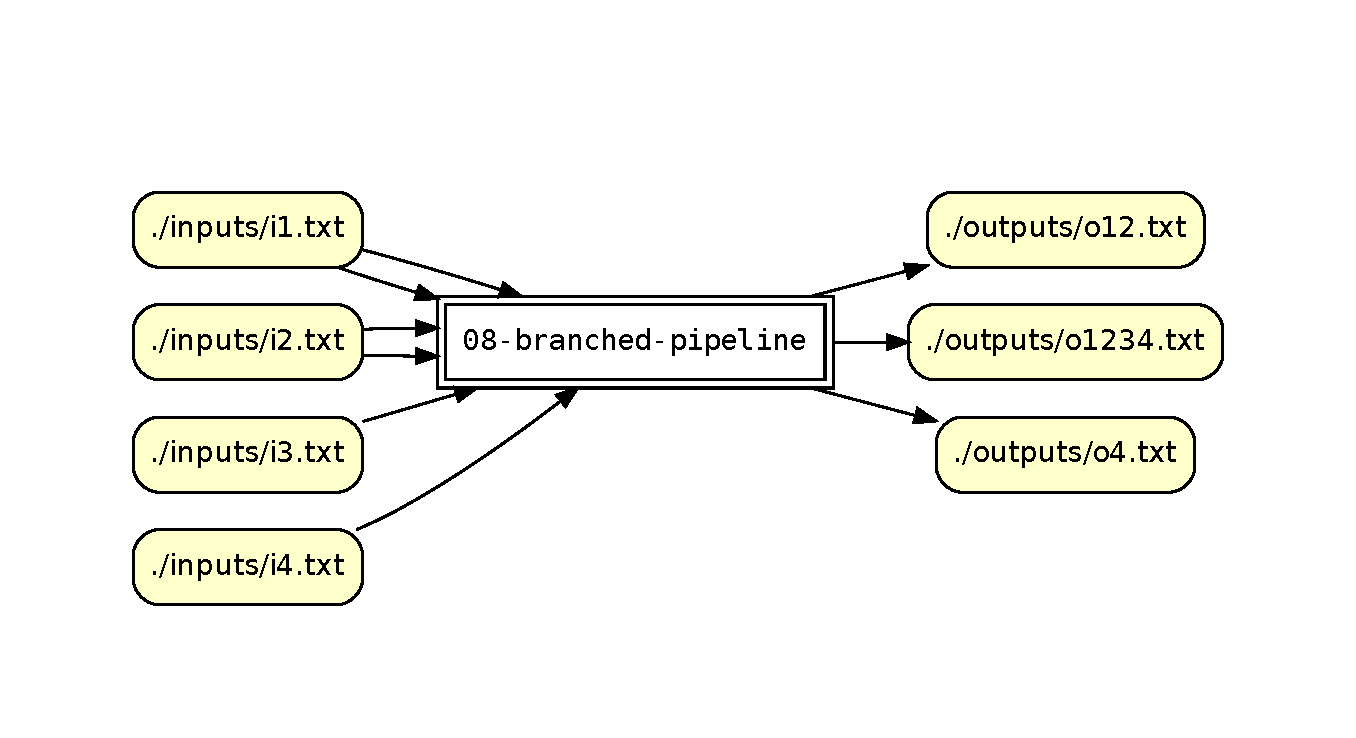
\includegraphics[width=\linewidth]{cpr_run_inputs_outputs.pdf}
            \caption{Visualization of inputs and outputs of the run as a whole.}
        \end{subfigure} 

\vspace*{1em}

    \begin{subfigure}[b]{1.0\linewidth}
        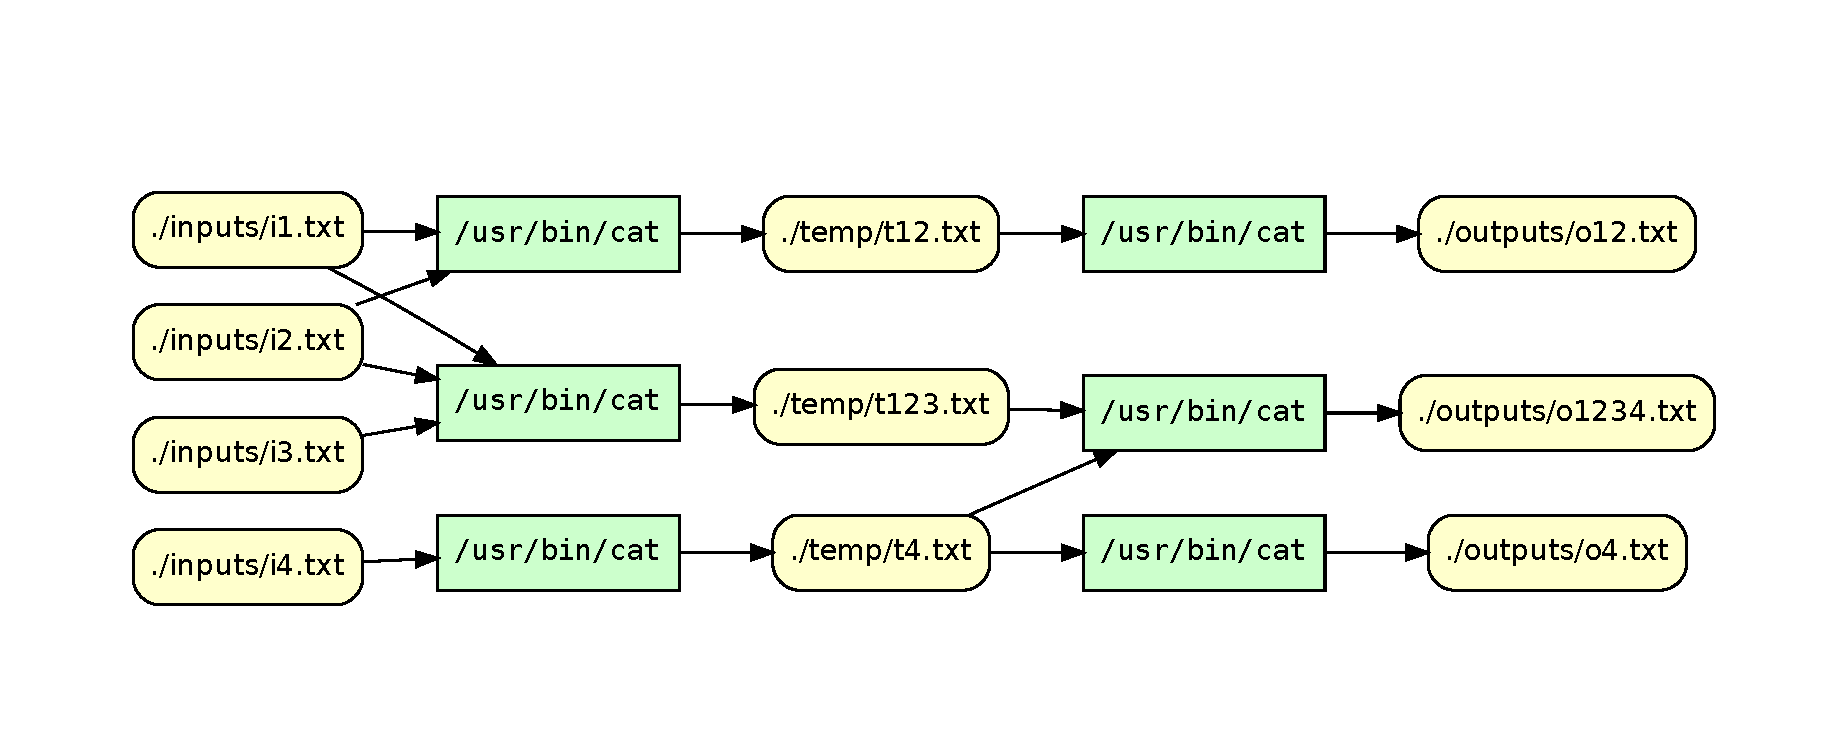
\includegraphics[width=\linewidth]{cpr_processes_and_data_files.pdf}
        \caption{Flow of data files through processes comprising the run.}
    \end{subfigure}
    \label{fig:cpr-example}
\end{figure}





